\documentclass[11pt]{article}
\usepackage{booktabs}
\usepackage[table]{xcolor}
\usepackage{tabularx}
\usepackage[a4paper,top=0.3in,bottom=0.75in,left=0.75in,right=0.75in]{geometry}
\usepackage{fontspec}
\usepackage{hyperref}
\usepackage{enumitem}
\usepackage{setspace}
\usepackage{mdframed}
\usepackage{graphicx}
\usepackage{float}
\usepackage{needspace}
\usepackage{tikz}
\usepackage{xspace}
\usetikzlibrary{arrows.meta,positioning,shapes.geometric}

\defaultfontfeatures{Ligatures=TeX,Scale=MatchLowercase}
\setmainfont{Arial}
\setsansfont{Arial}
\setmonofont{Menlo}

\hypersetup{colorlinks=true,urlcolor=blue}
\setlength{\parindent}{0pt}
\setlength{\parskip}{7pt}
\setlength{\emergencystretch}{2em}

\definecolor{ink}{RGB}{26,26,46}
\definecolor{muted}{RGB}{120,120,120}
\definecolor{gold}{RGB}{153,113,40}
\definecolor{headingblue}{RGB}{28,78,150}
\definecolor{linegray}{RGB}{220,220,220}

\newcommand{\sectionlabel}[1]{\textcolor{gold}{\textbf{\fontsize{11pt}{13pt}\selectfont #1}}}
\newcommand{\mainheading}[1]{\par\vspace{10pt}\noindent{\fontsize{15pt}{18pt}\selectfont\textcolor{headingblue}{#1}}
\par\vspace{4pt}}
\newcommand{\issueseventythree}{\href{https://github.com/LF-Decentralized-Trust-Mentorships/mentorship-program/issues/73}{Issue \#73}\xspace}
\newenvironment{auditpanel}[1]{%
\begin{mdframed}[linewidth=1pt,linecolor=linegray,backgroundcolor=gray!6,roundcorner=4pt,innertopmargin=8pt,innerbottommargin=8pt,innerleftmargin=10pt,innerrightmargin=10pt]
\textbf{#1}\par\vspace{2pt}
}{%
\end{mdframed}
}

\begin{document}

\color{ink}
{\LARGE\textbf{Darshit Khandelwal}}\\
{\small\textcolor{muted}{darshit2308@gmail.com | \href{https://github.com/darshit2308}{github.com/darshit2308} | IST (UTC +5:30)}}\\[-6pt]
\rule{\linewidth}{0.5pt}

\begin{tabularx}{\linewidth}{@{}X X@{}}
\sectionlabel{Applying for} & \sectionlabel{Addressed to} \\
\textbf{Hiero: GitHub Workflow App} & \textbf{Sophie Bulloch (exploreriii)} \\
\issueseventythree | LF Decentralized Trust & LF Decentralized Trust Mentorship Program
\end{tabularx}

\vspace{-5pt}
\rule{\linewidth}{0.4pt}

\textit{Dear Sophie Bulloch and the LF Decentralized Trust Mentorship Program,}

\nopagebreak[4]

% ─────────────────────────────────────────────────────────────
{\fontsize{15pt}{18pt}\selectfont\textcolor{gold}{How I found this program}}

I discovered the LFDT Mentorship Program in early March 2026 while searching for open-source projects focused on improving maintainer experience and automation capabilities. When \issueseventythree was published, I immediately resonated with the challenges described regarding contributor onboarding and workflow management. That same week, I began exploring the \texttt{hiero-sdk-cpp} repository, experimenting with its existing bot scripts to understand how maintainers were currently handling these issues.  

{\fontsize{15pt}{18pt}\selectfont\textcolor{gold}{Why I am interested}}

My interest in this project stems from directly observing the friction of scaling repository automation during my contributions to Hiero. When working on the \texttt{/unassign} command, I recognized the immediate value of these tools for maintainers but also noticed that propagating one logic fix could require opening near-identical PRs across multiple repositories because the workflow YAML and supporting scripts are distributed per repo. The public discussion on \issueseventythree reinforced that the real challenge is not merely adding more automation, but designing a system that is flexible, reusable, secure, and maintainable across repositories. That blend of research, architecture, and careful implementation is exactly the kind of problem I want to work on.

{\fontsize{15pt}{18pt}\selectfont\textcolor{gold}{Relevant experience \& skills}}

I have contributed to the Hiero ecosystem through multiple pull requests: \href{https://github.com/hiero-ledger/hiero-sdk-cpp/pull/1246}{PR \#1246}, \href{https://github.com/hiero-ledger/hiero-sdk-cpp/pull/1365}{PR \#1365}, \href{https://github.com/hiero-ledger/hiero-sdk-cpp/pull/1409}{PR \#1409}, \href{https://github.com/hiero-ledger/hiero-sdk-cpp/pull/1468}{PR \#1468}, and \href{https://github.com/hiero-ledger/hiero-sdk-cpp/pull/1494}{PR \#1494} in \textit{hiero-sdk-cpp} (assignment automation hardening), \href{https://github.com/hiero-ledger/hiero-did-sdk-js/pull/57}{PR \#57} in \textit{hiero-did-sdk-js} (timeout diagnostics), and \href{https://github.com/hiero-ledger/heka-identity-platform/pull/22}{PR \#22} plus \href{https://github.com/hiero-ledger/heka-identity-platform/pull/25}{PR \#25} in Heka Identity Platform (OID4VCI correctness and route fixes). I am also actively working on \href{https://github.com/hiero-ledger/heka-identity-platform/pull/69}{PR \#69} to persist wallet public DIDs and align Admin wallet IDs, and contributed \href{https://github.com/hiero-hackers/analytics/pull/158}{PR \#158} in hiero-hackers/analytics to expand maintainer telemetry.

Moreover, I built an end-to-end MVP of the contributor verification system for Issue \#87: \href{https://github.com/darshit2308/heka-identity-prototype}{heka-identity-prototype}, covering onboarding, credential handling, and verification flows.

I also developed a custom Probot service (\href{https://github.com/darshit2308/hiero-workflow-probot}{hiero-workflow-probot}) for GitHub workflow automation (PR labeling, milestone tracking, large PR warnings, automated responses), and extended it by porting on-comment logic from the hiero-sdk-cpp. While working on this, I identified a gap in handling stale issue assignments and proposed an automated reassignment approach, later reflected in workflow improvements.

Additionally, I have built decentralized identity systems, including a KYC platform using Groth16 ZK proofs and IPFS storage, along with Web3 applications such as \href{https://devfolio.co/projects/veilpad-2991}{VeilPad (1st place)} and \href{https://taikai.network/swellchain/hackathons/Swell-City-Buildathon/projects/cma45ss5e0c8dne4ug62e5j1g/idea}{Arden (restaking infrastructure track winner)}. These experiences give me strong familiarity with identity systems, cryptographic verification, backend architecture, and real-world integration challenges relevant to this project.

\par
\vspace{4pt}
{\fontsize{15pt}{18pt}\selectfont\textcolor{gold}{What I hope to gain}}

My goal during this mentorship is to transition from building MVPs to delivering production-grade services that maintainers can safely trust. I want to learn how experienced maintainers model security boundaries for applications interacting directly with repository workflows, how they scope and roll out architectural changes incrementally, and how they keep decisions transparent and auditable. I hope to use this mentorship to deepen those instincts and prepare myself to take long-term ownership of this kind of infrastructure.

\par
\noindent{\fontsize{13pt}{16pt}\selectfont\textcolor{gold}{\textbf{Please see the attached pages for my complete technical architecture, security model, configuration design, and phased implementation timeline for \issueseventythree.}}}

\vspace{4pt}
\textit{With deep respect,}\\[2pt]
{\fontsize{19pt}{23pt}\selectfont\textbf{Darshit Khandelwal}}
\clearpage

% ═══════════════════════════════════════════════════════════════
\begin{center}
{\small\textcolor{muted}{Mentorship Application}}\\[4pt]
{\fontsize{18pt}{22pt}\selectfont\textcolor{headingblue}{LFDT Mentorship Application: Hiero GitHub Workflow App (\issueseventythree)}}\\[6pt]
\rule{0.84\linewidth}{0.5pt}
\end{center}
% ═══════════════════════════════════════════════════════════════

\vspace{2pt}
{\fontsize{15pt}{18pt}\selectfont\textcolor{headingblue}{1. Executive Summary and Problem Statement}}

\vspace{4pt}

Currently, Hiero relies on a decentralized pattern of GitHub Actions and standalone JavaScript files to manage contributor workflows. While effective for individual repositories, this approach creates friction as the ecosystem scales. Updating a single automation rule currently requires identical pull requests across multiple repositories. This fragmentation makes consistent policy enforcement, security auditing, and horizontal scaling a significant administrative burden.

Following the architectural direction discussed in the community, I propose exploring a structured, hybrid workflow architecture that combines a centralized GitHub App (for orchestration and policy enforcement) with GitHub Actions (for isolated execution). In this model, core logic is centralized, and individual repositories opt into supported capabilities via a simple \texttt{.github/hiero-workflow.yml} configuration file. This separation of responsibilities could reduce duplicated logic, simplify rollout, and provide a clearer place to enforce permissions and auditability.

To validate the core mechanics of this transition, I researched and developed \texttt{hiero-workflow-probot}, an exploratory MVP that centralizes the \texttt{/assign} and \texttt{/unassign} logic from the C++ SDK and experiments with a PR validation pipeline. Building this prototype helped me explore GitHub's webhook payloads, Octokit API limitations, and permission boundaries before turning those lessons into a more measured production proposal.

During the mentorship, my focus will be to turn that research into a production-appropriate design and implementation path. Aligning with the project's core requirements, I will prioritize rigorous security hardening, comprehensive test coverage (unit, integration, and failure-path), transparent auditability for maintainer trust, and a safe, phased rollout strategy across the Hiero organization.
\vspace{5pt}
\noindent\textbf{Measurable Success Criteria for this Mentorship:}
\begin{itemize}[leftmargin=18pt,itemsep=2pt,topsep=0pt]
    \item \textbf{Reduced Maintenance Friction:} Updating a core bot rule (e.g., modifying the \texttt{/assign} regex) drops from requiring 12+ PRs across repositories to exactly 1 PR in the centralized service.
    \item \textbf{Zero CI Disruption:} The App maintains a 99\% uptime during the canary phase without blocking any legitimate maintainer merges.
    \item \textbf{Coverage Target:} The core orchestration logic and hybrid handoff mechanisms achieve strict 90\%+ unit/integration test coverage before organization-wide rollout.
\end{itemize}

To use the project's established framing: the existing Python SDK scripts represent V0 of this automation. The C++ SDK's refactored architecture represents V1. This proposal defines V2, a centralized GitHub App that replaces per-repository execution with a single hybrid orchestration service.


\mainheading{2. Pre-Application Contributions \& Ecosystem Alignment}

% ── CONTRIBUTION 1 ──────────────────────────────────────────
\textbf{1. Workflow Automation \& Bot Architecture}

\textbf{Repository:} hiero-sdk-cpp (\href{https://github.com/hiero-ledger/hiero-sdk-cpp/pull/1246}{PR \#1246}, \href{https://github.com/hiero-ledger/hiero-sdk-cpp/pull/1365}{PR \#1365}, \href{https://github.com/hiero-ledger/hiero-sdk-cpp/pull/1409}{PR \#1409}, \href{https://github.com/hiero-ledger/hiero-sdk-cpp/pull/1468}{PR \#1468}, \href{https://github.com/hiero-ledger/hiero-sdk-cpp/pull/1494}{PR \#1494} : Merged)

Before proposing architectural changes, I deeply immersed myself in the existing decentralized bot workflows. 

I implemented the \texttt{/unassign} command (\href{https://github.com/hiero-ledger/hiero-sdk-cpp/pull/1246}{PR \#1246}), introducing strict permission validation, issue state verification, and automated label reversion, all backed by targeted unit tests. 

In \href{https://github.com/hiero-ledger/hiero-sdk-cpp/pull/1365}{PR \#1365} and \href{https://github.com/hiero-ledger/hiero-sdk-cpp/pull/1409}{PR \#1409}, I hardened assignment safety by removing TOCTOU race conditions and revalidating stale label state before assignment. In \href{https://github.com/hiero-ledger/hiero-sdk-cpp/pull/1468}{PR \#1468}, I removed the \texttt{kind} label requirement to reduce friction, and in \href{https://github.com/hiero-ledger/hiero-sdk-cpp/pull/1494}{PR \#1494}, I added a needs-review bypass so top contributors are not blocked by the assignment cap. These improvements required careful handling of production automation constraints, ensuring backward compatibility while improving maintainer experience. 

This demonstrates my ability to safely evolve live CI/CD workflows without disrupting existing contributor processes.

% ── CONTRIBUTION 2 ──────────────────────────────────────────
\textbf{2. Systems Debugging \& Protocol Correctness}

\textbf{Repositories:} hiero-did-sdk-js (\href{https://github.com/hiero-ledger/hiero-did-sdk-js/pull/57}{PR \#57}), heka-identity-platform (\href{https://github.com/hiero-ledger/heka-identity-platform/pull/22}{PR \#22}, \href{https://github.com/hiero-ledger/heka-identity-platform/pull/25}{PR \#25} : Merged; \href{https://github.com/hiero-ledger/heka-identity-platform/pull/69}{PR \#69} : Open)

Beyond automation, I contributed to debugging distributed systems and protocol-level logic across the LFDT ecosystem. 

I improved observability in Hedera mirror node polling (\href{https://github.com/hiero-ledger/hiero-did-sdk-js/pull/57}{PR \#57}), resolved complex issues in OID4VCI credential flows and API routing (\href{https://github.com/hiero-ledger/heka-identity-platform/pull/22}{PR \#22}, \href{https://github.com/hiero-ledger/heka-identity-platform/pull/25}{PR \#25}), and am currently addressing wallet DID persistence and shared Admin wallet ID alignment (\href{https://github.com/hiero-ledger/heka-identity-platform/pull/69}{PR \#69}, open).

These contributions highlight my ability to rapidly onboard into complex codebases, identify root causes in distributed environments, and enforce correctness in protocol-driven systems.

% ── CONTRIBUTION 3 ──────────────────────────────────────────
\textbf{3. Ecosystem Analytics \& Telemetry}

\textbf{Repository:} hiero-hackers/analytics (\href{https://github.com/hiero-hackers/analytics/pull/158}{PR \#158 : Merged}, closes Issue \#131)

I contributed to establishing baseline telemetry for repository health and workflow visibility, enabling more data-driven decision-making for maintainers. I also participated in the \href{https://github.com/hiero-ledger/hiero-website/discussions/326}{hiero-website design discussion \#326}, proposing a React/Canvas-based hero refresh with gradients, gentle animations, and a tabbed contributor hub to reduce page length.

This work reflects my understanding that scalable systems require not only automation but also observability to monitor and continuously improve ecosystem performance.

% ── CONTRIBUTION 4 ──────────────────────────────────────────
\textbf{4. Review Queue Automation Architecture}

\textbf{Repository:} hiero-sdk-python (\href{https://github.com/hiero-ledger/hiero-sdk-python/issues/2229}{Issue \#2229 : In Progress}, \href{https://github.com/hiero-ledger/hiero-sdk-python/pull/2242}{PR \#2242 : Open})

Following mentorship initiation, I raised a concrete architectural proposal for automating the Python SDK's review queue management and addressing the pain point that directly mirrored the cross-repository automation challenges outlined in \issueseventythree. I designed a 4-phase iterative implementation plan (Foundation + Label Sync → Difficulty-Based Routing → Assignment, Comments + Escalation → Changes-Requested Handling).

This demonstrates my ability to bridge exploratory prototypes into actionable, mentor-guided production work aligned with real ecosystem pain points.

\textbf{Pre-Mentorship Progress Update:}
\begin{itemize}[leftmargin=18pt,itemsep=2pt,topsep=2pt]
    \item Opened \href{https://github.com/hiero-ledger/hiero-sdk-python/issues/2229}{Issue \#2229} with mentor feedback and iterative refinement.
    \item Submitted \href{https://github.com/hiero-ledger/hiero-sdk-python/pull/2242}{PR \#2242} implementing Phase 1 (Foundation + Label Sync).
    \item Merged \href{https://github.com/hiero-hackers/analytics/pull/158}{PR \#158} in hiero-hackers/analytics, closing Issue \#131.
    \item Shipped five merged PRs in hiero-sdk-cpp hardening assignment automation (\href{https://github.com/hiero-ledger/hiero-sdk-cpp/pull/1246}{PR \#1246}, \href{https://github.com/hiero-ledger/hiero-sdk-cpp/pull/1365}{PR \#1365}, \href{https://github.com/hiero-ledger/hiero-sdk-cpp/pull/1409}{PR \#1409}, \href{https://github.com/hiero-ledger/hiero-sdk-cpp/pull/1468}{PR \#1468}, \href{https://github.com/hiero-ledger/hiero-sdk-cpp/pull/1494}{PR \#1494}).
    \item Participated in Python SDK PR reviews (\#2194, \#2170, \#2213), earning direct maintainer recognition.
\end{itemize}

% ── SUMMARY ──────────────────────────────────────────
\textbf{Summary of Capability:}

By enhancing production bot workflows, building exploratory orchestration prototypes, contributing to observability work, and debugging protocol-level systems across multiple repositories, I have developed both the ecosystem familiarity and the engineering discipline needed to execute \issueseventythree thoughtfully.
\mainheading{3. Exploratory Prototypes (The Research Phase)}

\vspace{5pt}
To validate the architectural challenges of centralizing Hiero's workflows, I did not want to rely strictly on theory. Instead, I built two targeted GitHub App prototypes to test different aspects of the proposed system: policy orchestration and legacy logic porting.

\vspace{5pt}
\noindent
\textbf{Prototype 1: Orchestration \& Dynamic Configuration}
\begin{itemize}[leftmargin=18pt,itemsep=2pt,topsep=2pt]
\item \textbf{Repository:} \href{https://github.com/darshit2308/hiero-workflow-probot}{darshit2308/hiero-workflow-probot} \newline
\textbf{Demo:} \href{https://youtu.be/P9EdRm2D2v8}{Demo video}
\item \textbf{Focus:} Testing how a centralized app interacts with a repository-level configuration file. \newline
\texttt{.github/hiero-workflow.yml}
\item \textbf{Working Features:} This app reads repository config to post greeting messages, auto-label PRs, enforce PR size warnings, and manage milestone tracking. It shows that orchestration behavior can be driven from one config file instead of custom application code in each repository.
\end{itemize}

\vspace{5pt}
\noindent
\textbf{Prototype 2: Porting Hiero's Business Logic}
\begin{itemize}[leftmargin=18pt,itemsep=2pt,topsep=2pt]
\item \textbf{Repository:} \href{https://github.com/darshit2308/heiro-probot-official}{darshit2308/heiro-probot-official} | \textbf{Demo:} \href{https://youtu.be/EVA5NBKnafA}{Demo video}
\item \textbf{Focus:} Testing whether Hiero's highly specific, tightly coupled workflow scripts can actually survive outside of the GitHub Actions shell.
\item \textbf{Working Features:} I successfully ported the official C++ SDK's \texttt{on-comment} logic into a Node.js Probot environment. This handles the complex \texttt{/assign} and \texttt{/unassign} routines, including skill-tier checks and assignment limits, entirely through the Octokit API rather than local repository execution.
\end{itemize}

\vspace{5pt}
\noindent
\textbf{What this means for the Mentorship (The V2 Build):} \\
These prototypes show that several core mechanics are promising: dynamic configuration can work, and the assignment logic can be moved out of a single repository's shell scripts. The goal for the mentorship period is to refine those learnings into a secure, testable, and maintainable hybrid architecture that balances centralized orchestration with GitHub Actions for execution where appropriate.

\mainheading{4. Codebase Analysis and Architecture Findings}

\subsection*{4.1 The Limits of the Current Per-Repo Setup}

Studying the workflow execution patterns in the C++ SDK, alongside the mentor's guidance about scaling across repositories, revealed a clear maintenance challenge. Today, key maintainer logic lives in standalone YAML triggers and JavaScript handlers nested within repository-local workflow setups. 

To patch a single edge case in the bot's parsing logic, maintainers may need to duplicate and review similar pull requests across multiple projects. As the ecosystem scales horizontally, this decentralized model creates unnecessary coordination cost. A centralized policy layer is therefore a strong candidate for reducing that burden, provided it is designed with repository-specific controls and a safe rollout model.

% ── TABLE: Current state vs proposed state ───────────────────
\begin{table}[H]
\centering
\renewcommand{\arraystretch}{1.3}
\begin{tabularx}{\textwidth}{@{} l X X @{}}
\toprule
\textbf{Dimension} & \textbf{Current (Per-Repo)} & \textbf{Proposed (Hybrid App Architecture)} \\
\midrule
Install on new repo & Multiple workflow files and helper scripts to align & App installation plus lightweight repository config \\
Update logic & Similar PRs across multiple repositories & Centralized service update plus controlled rollout \\
Feature toggles & Limited and repository-local & \texttt{.github/hiero-workflow.yml} \\
Audit trail & Split across workflow runs and comments & Centralized decision logs plus repository-visible status \\
Security model & Runner-scoped workflow permissions & App-scoped permissions with explicit handoff to Actions \\
Horizontal scaling & Higher coordination cost & Lower coordination cost if rollout is staged carefully \\
\bottomrule
\end{tabularx}
\end{table}

\subsection*{4.2 The Target: A Hybrid Architecture (App + Actions)}

While my prototypes ran entirely in Probot, building a monolithic Node.js server to handle every single compute task is an anti-pattern for a project of Hiero's scale. Aligning with the mentor's vision, the production V2 system must utilize a \textbf{structured, hybrid approach}:
\begin{itemize}[leftmargin=18pt,itemsep=2pt,topsep=2pt]
    \item \textbf{GitHub App (Orchestration \& Policy):} A centralized Node.js service listens to webhooks. It reads the specific repository's \texttt{.yml} policy, makes instant state decisions (like rejecting an assignment if limits are reached), and handles lightweight API interactions.
    \item \textbf{GitHub Actions (Execution):} For heavy, compute-intensive tasks (like compiling code, running deep cryptographic checks, or analyzing source files), the App dispatches a \texttt{repository\_dispatch} event to trigger an isolated Action natively within the target repository. 
\end{itemize}
This separation of responsibilities keeps the central server lightweight and resilient, while safely leveraging GitHub's native CI infrastructure for heavy execution.

\subsection*{4.3 Security Boundaries and Pull Request Injection}

The present decentralized approach is heavily encumbered by its dependency on the standard GitHub Actions execution context. If a workflow relies on the \texttt{pull\_request\_target} event to operate with elevated access on untrusted fork payloads, it introduces a well-documented injection risk. 

A centralized GitHub App model structurally mitigates this class of risk. The App intercepts the webhook externally, verifies it via HMAC-SHA256 signatures, and evaluates the payload in an isolated environment with strictly scoped, least-privilege token access before deciding whether any downstream workflow should run.

\subsection*{4.4 Configuration Layering Design}

Because different repositories possess varying maturity levels, enforcing a single global policy would be risky for legacy projects. My proposed contract for handling that variation is the \texttt{.github/hiero-workflow.yml} file.
When the centralized App receives an event, it fetches this configuration first. Maintainers can manipulate simple boolean switches and numerical thresholds to adjust repository behavior instantly, without touching a single line of JavaScript.

% ── CODE BLOCK: hiero-workflow.yml schema ────────────────────
\begin{verbatim}
# .github/hiero-workflow.yml
workflows:
  assign:
    enabled: true
    max_open_assignments: 2
    enforce_skill_progression: true
  pr_pipeline:
    require_dco: true
    require_gpg: true
    size_warnings_enabled: true
  stale_assignments:
    enabled: false
    warning_days: 21
    auto_unassign_days: 28
audit:
  log_level: structured
  retention_days: 90
\end{verbatim}

\subsection*{4.5 Auditability and Transparency}

If the automation removes a contributor from an issue, a human maintainer needs to easily find out \textit{why}. The centralized App will integrate a deterministic structured audit log (e.g., recorded natively via GitHub Check Runs or a dedicated administrative repository). Every time the bot acts, it records the repository, the trigger event, the specific \texttt{.yml} rule that was evaluated, and the final outcome. This ensures the automation remains transparent, establishing uncontested rationale over the workflow pipeline.

\subsection*{4.6 Safe Rollout Strategy}

Migrating established workflows demands extreme systematic caution to prevent operational friction. I propose an incremental deployment path governed by enforcement modes. New repository integrations can opt into a passive 'warn-only' state that outputs diagnostic pipeline metrics without forcefully overriding assignments or halting merges. Active canary deployments will strictly target the \texttt{hiero-sdk-cpp} repository as our initial testing ground before pursuing broader organization-wide integration.

\subsection*{4.7 Extensibility and Future Workflow Design}

As Hiero's administrative complexity grows, the automation service must adapt without causing systemic regressions. I would therefore use a modular architecture where new maintainer capabilities are added as isolated integrations subscribing to the central routing core, keeping foundational assignment and validation logic stable while the system evolves over time.

\subsection*{4.8 Alternatives Considered \& Architectural Tradeoffs}

Before proposing the Hybrid App architecture, I evaluated solving this using GitHub's native "Reusable Workflows." 
\begin{itemize}[leftmargin=18pt,itemsep=2pt,topsep=0pt]
    \item \textbf{The Reusable Workflow Alternative:} Centralizing the YAML files into a single \texttt{.github} repository and calling them remotely from the SDKs.
    \item \textbf{Why it was rejected:} The primary technical blocker is that \texttt{workflow\_call} cannot auto-checkout shared script files from a centralized repository—callee workflows do not inherit file access from the caller. This means supporting scripts (e.g., \texttt{.scripts/on-comment.js}) would either need to be duplicated per repository or fetched at runtime, undermining centralization. Beyond this concrete limitation, Reusable Workflows also retain the \texttt{pull\_request\_target} injection risks because they execute inside the target repository's CI runner, and they lack persistent state, making complex orchestration (like cross-repo assignment limits or queued concurrent comments) nearly impossible. The solution is a proper JavaScript Action, which GitHub auto-downloads and executes in isolation. This is the structure being implemented in the pre-mentorship phase, where the review-sync logic in hiero-sdk-python is written as a clean JavaScript module designed for extraction into a proper GitHub Action in hiero-hackers during Milestone 1.
    \item \textbf{The Hybrid Tradeoff:} The tradeoff of my proposed App architecture is the introduction of a new hosting dependency (the Node.js server). I acknowledge this adds infrastructure overhead for LFDT, which is why my focus is strictly on making the service lightweight and rigorously tested, treating the GitHub API as the single source of truth for state to minimize infrastructure overhead.
\end{itemize}


\subsection*{4.9 Architectural Tradeoffs: Probot vs. GitMesh}

The updated requirements for Issue \#73 introduce the possibility of AI-based PR reviewing. In evaluating the architecture for this, I researched \texttt{LF-Decentralized-Trust-labs/gitmesh}, which solves similar orchestration problems using a Policy-as-Code approach via OPA (Open Policy Agent). 

While GitMesh's OPA approach is genuinely impressive for complex AI governance and multi-agent scenarios, a Probot foundation remains the most appropriate choice for this project's immediate V2 phase. The core requirements (DCO enforcement, GPG checks, assignment limits) are deterministic compliance layers; they require 100\% reliability and are non-negotiable. 

By building a lightweight, deterministic Probot core first, the architecture makes it straightforward to plug in advanced, AI-based workflows (potentially integrating GitMesh concepts) as isolated API calls on top of the foundational layer when the ecosystem is ready for them.


\mainheading{5. Visual Architecture and Data Flows}

This section visually contrasts the operational bottlenecks of the current decentralized scripts against the optimized, secure routing of the proposed hybrid architecture. 

\vspace{10pt}
\noindent\textbf{Current State: Fragmented Per-Repo Architecture}

% ── FIGURE 2: BEFORE DIAGRAM ─────────────────────────────────

\begin{figure}[H]
\centering
\includegraphics[width=0.95\textwidth]{figure2.png}
\caption{Current per-repo architecture. Each Hiero repository maintains its own local workflow YAML files and supporting bot scripts, so even small logic changes can require repeated updates across multiple repositories.}
\end{figure}

\vspace{10pt}
\noindent\textbf{Target State: Hybrid GitHub App Architecture}

% ── FIGURE 3: AFTER DIAGRAM ──────────────────────────────────
\begin{figure}[H]
\centering
\includegraphics[width=0.95\textwidth]{figure3.png}
\caption{Target hybrid architecture. The central Probot App handles webhook orchestration and policy evaluation while delegating heavier execution tasks back to isolated GitHub Actions. The intent is to centralize policy without over-centralizing execution.}
\end{figure}

\vspace{10pt}
\noindent\textbf{PR Check Validation Pipeline — Execution Flow (See Figure \ref{fig:pipeline})}

% ── FIGURE 4: PR PIPELINE FLOW ───────────────────────────────
\begin{figure}[H]
\centering
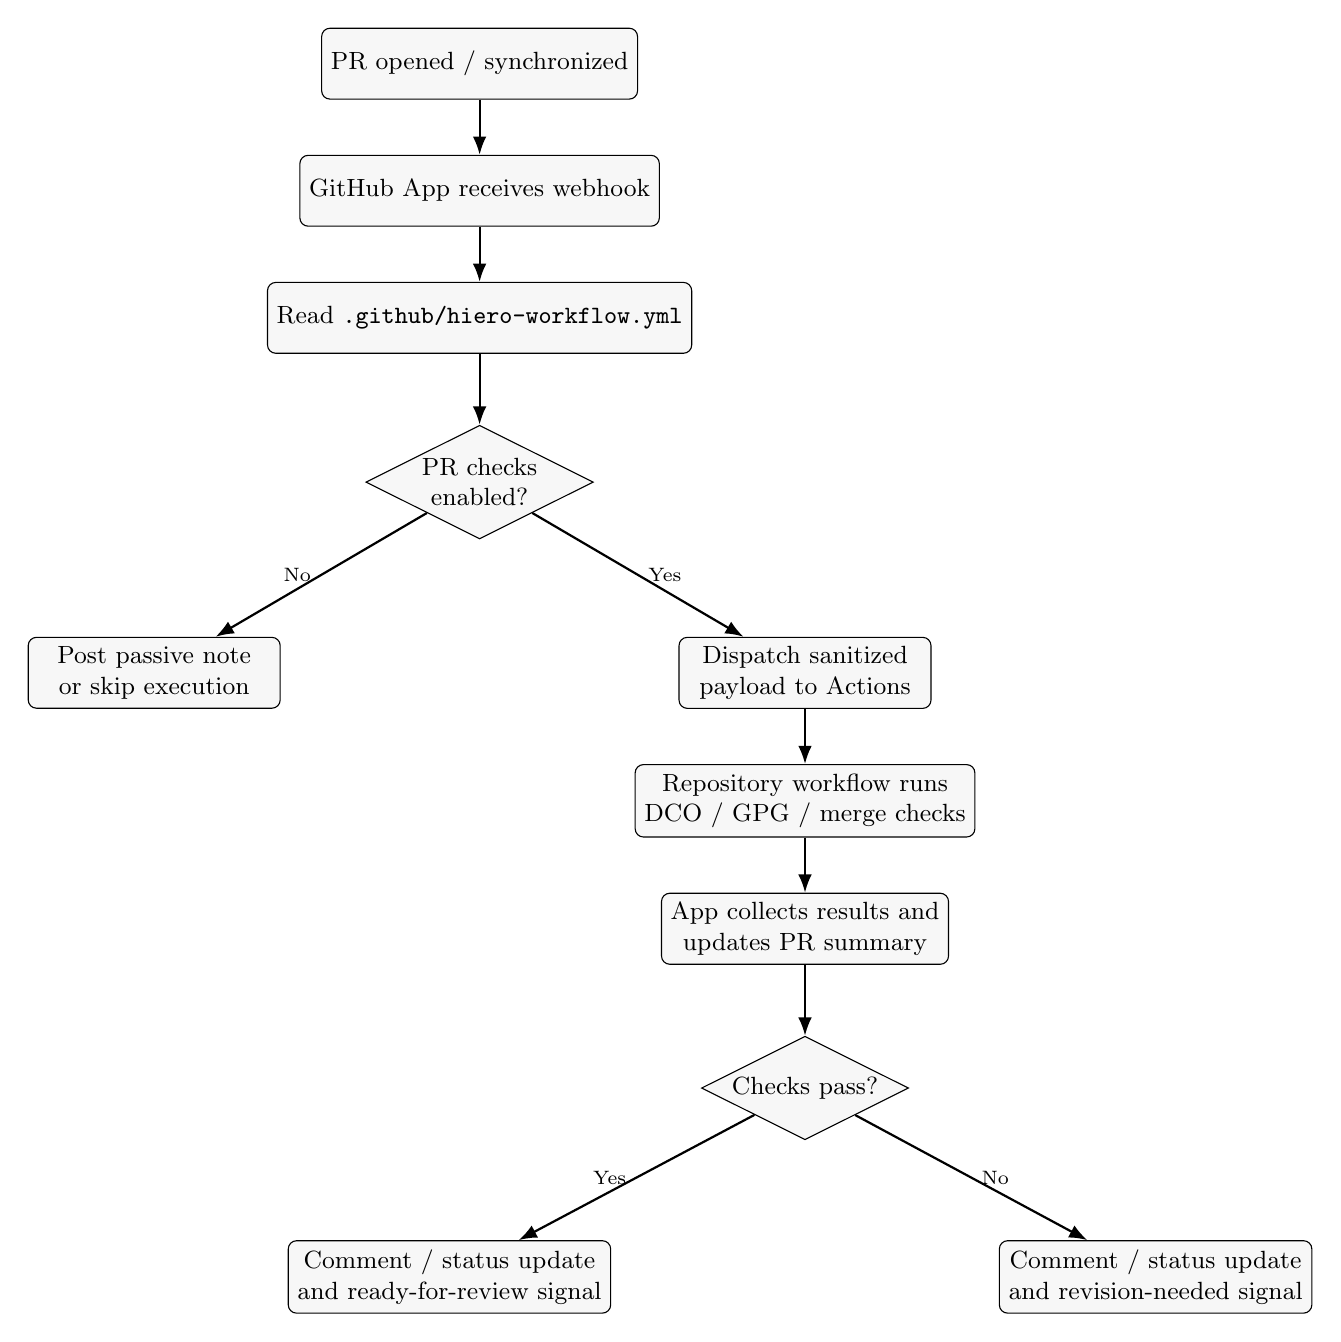
\begin{tikzpicture}[
    node distance=7mm and 10mm,
    every node/.style={font=\small, align=center},
    box/.style={draw, rounded corners=3pt, minimum width=3.2cm, minimum height=0.9cm, fill=gray!6},
    decision/.style={draw, diamond, aspect=2, inner sep=1pt, fill=gray!6},
    line/.style={-Latex, thick}
]
\node[box] (event) {PR opened / synchronized};
\node[box, below=of event] (router) {GitHub App receives webhook};
\node[box, below=of router] (config) {Read \texttt{.github/hiero-workflow.yml}};
\node[decision, below=of config, yshift=-2mm] (enabled) {PR checks\\enabled?};
\node[box, below left=16mm and 18mm of enabled] (skip) {Post passive note\\or skip execution};
\node[box, below right=16mm and 18mm of enabled] (dispatch) {Dispatch sanitized\\payload to Actions};
\node[box, below=of dispatch] (actions) {Repository workflow runs\\DCO / GPG / merge checks};
\node[box, below=of actions] (status) {App collects results and\\updates PR summary};
\node[decision, below=of status, yshift=-2mm] (pass) {Checks pass?};
\node[box, below left=16mm and 18mm of pass] (approve) {Comment / status update\\and ready-for-review signal};
\node[box, below right=16mm and 18mm of pass] (revise) {Comment / status update\\and revision-needed signal};

\draw[line] (event) -- (router);
\draw[line] (router) -- (config);
\draw[line] (config) -- (enabled);
\draw[line] (enabled) -- node[left, font=\scriptsize] {No} (skip);
\draw[line] (enabled) -- node[right, font=\scriptsize] {Yes} (dispatch);
\draw[line] (dispatch) -- (actions);
\draw[line] (actions) -- (status);
\draw[line] (status) -- (pass);
\draw[line] (pass) -- node[left, font=\scriptsize] {Yes} (approve);
\draw[line] (pass) -- node[right, font=\scriptsize] {No} (revise);
\end{tikzpicture}
\caption{A hybrid PR validation flow. The GitHub App handles webhook intake, policy decisions, and result reporting, while repository-local GitHub Actions execute the heavier validation steps.}
\label{fig:pipeline}
\end{figure}

\mainheading{6. Security Model}

Security cannot be an afterthought when designing an organization-wide automation service. Aligning directly with the requirement for the "thoughtful handling of permissions and safety," this hybrid architecture aims for a fail-closed security posture. By decoupling the event trigger from the execution environment, it can reduce several common CI/CD risks that would otherwise need to be handled inside repository workflows themselves.

\vspace{5pt}
\noindent
\textbf{1. Mitigating Pull Request Injection Risks}
\begin{itemize}[leftmargin=18pt,itemsep=2pt,topsep=0pt]
\item \textbf{The Vector:} Decentralized workflows often rely on the \texttt{pull\_request\_target} event to operate with elevated access on PRs from forks. This creates a severe injection vulnerability where untrusted fork code might execute within a trusted CI environment.
\item \textbf{The Hybrid Mitigation:} The GitHub App acts as a secure airgap. The App intercepts the untrusted webhook externally and evaluates the payload inside the isolated Node.js environment. When heavy execution is required, the App triggers a \texttt{repository\_dispatch} event to GitHub Actions, passing only sanitized, explicitly defined parameters. No untrusted fork code is ever blindly executed with elevated privileges.
\end{itemize}

\vspace{5pt}
\noindent
\textbf{2. Granular, Least-Privilege Permissions}
\begin{itemize}[leftmargin=18pt,itemsep=2pt,topsep=0pt]
\item \textbf{Required permissions:} Read/Write access on Issues and Pull Requests; Read-only access on Metadata and Contents.
\item \textbf{What is explicitly avoided where possible:} unnecessary access to repository secrets, workflow administration, or direct code-writing capabilities. The exact permission set should be minimized and validated during implementation.
\item \textbf{Why this matters:} Unlike Personal Access Tokens (PATs), which often grant repository-wide write access and represent a massive security liability, the GitHub App operates under restrictive cryptographic bounds. This strict least-privilege model drastically minimizes the blast radius in the unlikely event of a compromise.
\end{itemize}

\vspace{5pt}
\noindent
\textbf{3. Cryptographic Webhook Verification}
\begin{itemize}[leftmargin=18pt,itemsep=2pt,topsep=0pt]
\item To prevent payload spoofing or unauthorized API triggers, the App authenticates every incoming GitHub webhook using HMAC-SHA256 signatures derived from a private webhook secret. Any request failing this cryptographic validation is immediately dropped before processing.
\end{itemize}

\vspace{5pt}
\noindent
\textbf{4. Infinite Loop \& Rate Limit Protection}
\begin{itemize}[leftmargin=18pt,itemsep=2pt,topsep=0pt]
\item Automated systems are notoriously prone to feedback loops (e.g., a bot reacting to its own automated comment). The architecture should enforce actor-type validations and explicit bot guards so the app does not trigger its own workflows, reducing rate-limit exhaustion and runaway execution costs.
\end{itemize}

\vspace{5pt}
\noindent
\textbf{5. Concurrency and Race Condition Handling}
\begin{itemize}[leftmargin=18pt,itemsep=2pt,topsep=0pt]
\item The existing decentralized YAML workflows utilize \texttt{concurrency} groups to prevent race conditions when multiple \texttt{/assign} comments arrive simultaneously. The centralized Node.js service replicates this safety mechanism by implementing an asynchronous task queue keyed by the issue number, ensuring state mutations are processed sequentially and predictably.
\end{itemize}

\vspace{5pt}
\noindent
\textbf{6. Non-Repudiation and Auditability}
\begin{itemize}[leftmargin=18pt,itemsep=2pt,topsep=0pt]
\item Security requires visibility. Because the App centralizes decision-making, it inherently generates a unified, structured audit trail. Maintainers can trace exactly which user triggered an event, which \texttt{.yml} policy rule was evaluated, and what the final system action was, establishing total transparency over the automation pipeline.
\end{itemize}

\vspace{5pt}
\noindent
\textbf{7. Explicit Trust Boundaries \& Attack Surface}
\begin{itemize}[leftmargin=18pt,itemsep=2pt,topsep=0pt]
\item The primary attack surface is the webhook ingestion endpoint. We model threats where malicious actors spam issue comments to exhaust API limits or inject Malicious Markdown.
\item \textbf{Trust Boundary:} The App explicitly does \textit{not} trust the GitHub webhook payload. It validates the payload against a strict, predefined schema (rejecting unexpected fields) before passing parameters to the \texttt{repository\_dispatch} payload, ensuring that even if the App's parser is tricked, the repository-level GitHub Action receives neutralized inputs.
\end{itemize}

\vspace{5pt}
\noindent
\textbf{8. Fail-Safe Degradation (What happens if the App crashes?)}
\begin{itemize}[leftmargin=18pt,itemsep=2pt,topsep=0pt]
\item In the event of a total App outage, the repository does not lock up. Because the App only handles automation, human maintainers retain their native GitHub UI abilities to manually assign issues, apply labels, and merge PRs. The system is designed to fail gracefully into a manual state, never blocking critical repository operations.
\end{itemize}



\mainheading{7. Target Production Architecture}

Addressing the explicit requirement for a "clear separation of responsibilities" and a "maintainable and extensible structure," the Node.js Probot application is designed using a strictly modular, event-driven pattern. This ensures the central orchestration layer remains lightweight while effectively managing the hybrid handoff to GitHub Actions.

\vspace{5pt}
\noindent
\textbf{1. Module Separation and Responsibility Boundaries}
\begin{itemize}[leftmargin=18pt,itemsep=2pt,topsep=0pt]
\item \textbf{index.js (The Router):} The core Probot entry point. It securely ingests external webhooks and routes them to isolated validation handlers.
\item \textbf{config/:} Dedicated solely to reading, validating, and caching the declarative \texttt{.github/hiero-workflow.yml} configuration from the target repository.
\item \textbf{commands/:} Houses the isolated issue lifecycle logic (e.g., \texttt{/assign}, \texttt{/unassign}), bounded securely away from pull-request manipulation layers.
\item \textbf{services/dispatcher.js (The Hybrid Bridge):} The module responsible for the Hybrid Architecture handoff. It triggers \texttt{repository\_dispatch} events to initiate heavy CI/CD execution natively within GitHub Actions.
\item \textbf{helpers/api.js:} A centralized Octokit adapter that manages API rate limits, standardizes HTTP retries, and isolates network logic from business rules.
\end{itemize}

\vspace{5pt}
\noindent
\textbf{2. Error Handling and Fail-Safe Behaviour}
\begin{itemize}[leftmargin=18pt,itemsep=2pt,topsep=0pt]
\item \textbf{Standardized Responses:} Every validation gate returns a strictly typed \texttt{\{success, data, error\}} object. This reduces unhandled exceptions and makes failure behaviour more predictable.
\item \textbf{No Silent Failures:} Destructive state errors (e.g., failing to assign a user due to rate limits) do not fail silently in the backend logs. They trigger automated, informative diagnostic replies directly in the affected issue thread.
\item \textbf{Resilient Polling:} Implementing exponential backoff and timeout boundaries for repetitive tasks (like merge-conflict polling) ensures the app does not bottleneck its own event loop during high-traffic spikes.
\end{itemize}

\vspace{5pt}
\noindent
\textbf{3. Per-Repository Configuration Model}
\begin{itemize}[leftmargin=18pt,itemsep=2pt,topsep=0pt]
\item \textbf{Fail-Safe Defaults:} If a repository is integrated but lacks a valid \texttt{hiero-workflow.yml} file, the system defaults to a passive 'warn-only' state. It logs telemetry but performs no state mutations, preventing accidental disruptions.
\item \textbf{Granular Toggles:} Maintainers engage capabilities effortlessly via simple boolean feature flags. A maintainer can mandate strict GPG cryptographic signatures on one repository without forcing that requirement onto legacy repositories.
\item \textbf{Community Review Signal:} For GFI and beginner-difficulty PRs, the system applies a configurable label (e.g., \texttt{help-wanted: reviewer}) to signal that community review contributions are welcome, directly supporting the Python SDK's reviewer base expansion.
\end{itemize}

\vspace{5pt}
\noindent
\textbf{4. Extensibility Pattern}
\begin{itemize}[leftmargin=18pt,itemsep=2pt,topsep=0pt]
\item Because the app would use a modular, event-driven architecture, future expansion can happen with lower risk. New capabilities can be added as independent subscribers listening to \texttt{app.on()} events, adjacent to the existing baseline.
\item This keeps the core \texttt{/assign} and \texttt{/unassign} routing logic stable while additional maintainer workflows are explored in isolated modules.
\end{itemize}

\vspace{5pt}
\noindent
\textbf{5. Cross-Repository Rollout Strategy}
\begin{itemize}[leftmargin=18pt,itemsep=2pt,topsep=0pt]
    \item \textbf{Pre-Mentorship Phase: Direct SDK Implementation (hiero-sdk-python).} Before formal program initiation, I have begun a 4-phase iterative build directly in the Python SDK (Issue \#2229), establishing foundational patterns and validating concrete automation needs. This grounds the architecture in real repository pain points rather than pure theory.
    \item \textbf{Mentorship Phase 1: Abstraction to Centralized Action (hiero-hackers).} During the mentorship window, I will abstract the validated patterns from the Python SDK work into a proper, reusable JavaScript Action housed in the \texttt{hiero-hackers} organization. This ensures the central service is battle-tested against real ecosystem requirements before broader deployment.
    \item \textbf{Mentorship Phase 2: Canary Rollout (\texttt{hiero-sdk-cpp}).} With the abstracted architecture validated, I will deploy the centralized Action to the familiar, high-traffic C++ SDK environment to generate comprehensive impact validation and stress-test the concurrent queue under realistic load.
    \item \textbf{Mentorship Phase 3+: Organization-Wide Rollout.} Incrementally expanding to additional SDK repositories (e.g., \texttt{hiero-sdk-js}) once telemetry and maintainer feedback from the canary phase indicate stable behaviour.
    \item \textbf{Changes-Requested to Draft Pattern:} Align with the cpp bot-on-pr-review flow by converting PRs to draft on changes requested, minimizing label churn while keeping reviewer intent explicit.
\end{itemize}

\mainheading{8. Implementation Plan \& Milestones}

% Aligning with LFDT 2026 Program timeline (June 15 -- Nov 30).

\vspace{10pt}
\begin{table}[H]
\centering
\renewcommand{\arraystretch}{1.4}
\begin{tabularx}{\textwidth}{@{} >{\bfseries}l l X @{}}
\toprule
Phase & \textbf{Timeline} & \textbf{Engineering Focus \& Deliverables} \\
\midrule
Milestone 1 & Jun 15 -- Jul 15 &
\textbf{Core Orchestration \& Config Layer} \newline
Finalize the \texttt{hiero-workflow.yml} schema. Build the central Probot event router and dynamic configuration reader. \newline \textit{Deliverable:} Repositories can install the App, and the App correctly parses feature toggles per repository. \\

Milestone 2 & Jul 16 -- Aug 23 &
\textbf{Hybrid Pipeline \& Production Hardening} \newline
Build the dispatcher bridge for the hybrid architecture. Implement the PR validation engine (DCO, GPG, merge conflicts) utilizing the App-to-Actions handoff. Achieve comprehensive test coverage across core state mutations. \newline \textit{Deliverable:} The hybrid dispatcher bridge is functional; PR validation runs end-to-end with 90\%+ test coverage. \\

\rowcolor{gray!10}
Midterm & \textbf{Aug 24 -- 31} &
\textbf{Official Midterm Evaluation} \newline
Live demonstration of the hybrid PR pipeline and issue assignment logic running safely and deterministically within the \texttt{hiero-hackers} sandbox environment. \\
Milestone 3 & Sep 1 -- 30 &
\textbf{Audit Logging \& Observability} \newline
Implement the deterministic structured audit log to record all system actions. Build maintainer-facing diagnostics to easily trace why specific workflow decisions (e.g., assignment rejections) were made. \newline \textit{Deliverable:} Transparent, queryable audit trails are fully operational. \\

Milestone 4 & Oct 1 -- 31 &
\textbf{Canary Rollout \& Hardening} \newline
Deploy the App to \texttt{hiero-sdk-cpp} as a live canary. The primary focus here is stability: monitoring rate limit governors, verifying webhook signatures in production, and resolving edge cases. \newline \textit{Deliverable:} The App runs safely on the canary repo for 30 days without dropping webhook events or blocking legitimate PRs. \\

Milestone 5 & Nov 1 -- 14 &
\textbf{Stretch Goals: Stale Assignment \& Extensibility} \newline
\textit{If core stability is achieved ahead of schedule}, I will implement the cron-driven stale assignment worker and document extension hooks for future capabilities. \newline \textit{Deliverable:} Working stale-issue sweeper and documented plugin architecture. \\

\rowcolor{gray!10}
Final & \textbf{Nov 15 -- 30} &
\textbf{Official Final Evaluation \& Handoff} \newline
Deliver cross-organization adoption guides and maintainer documentation. Execute the final handoff demonstration, focusing on the core Hybrid PR pipeline. \\

\bottomrule
\end{tabularx}
\end{table}

\textbf{Deliverables Mapping to \issueseventythree}
\begin{itemize}[leftmargin=18pt,itemsep=2pt,topsep=2pt]
    \item \textbf{Reusable GitHub App for maintainer workflows:} Delivered in M1 and M2 via the core Node.js Probot service and the hybrid dispatcher bridge.
    \item \textbf{Configurable per-repository feature toggles:} Delivered in M1 via the dynamic YAML reader, allowing maintainers to control automation without writing code.
    \item \textbf{Tests covering core logic, workflow behaviour, and safety constraints:} Delivered in M2 and M4 through strict unit/integration testing and the live canary deployment.
    \item \textbf{Documentation for maintainers and contributors:} Delivered in the Final phase, ensuring smooth onboarding and cross-organizational adoption.
    \item \textbf{Recommendations and extension hooks for future workflows:} Delivered in M5 via documented integration boundaries for safely adding new maintainer capabilities.
\end{itemize}

\mainheading{9. Testing Strategy \& Execution Quality}

Acknowledging the mentor's guidance that safety and testing are "perhaps the most important part" of this initiative, the application will be developed under a strict Test-Driven Development (TDD) philosophy. The goal is to build absolute maintainer trust through a deterministic, layered validation strategy.

\vspace{5pt}
\noindent
\textbf{Testing Strategy (Layered Validation)}
\begin{itemize}[leftmargin=18pt,itemsep=2pt,topsep=2pt]
    \item \textbf{Unit Tests (Pure Logic):} Validating the stateless utility functions within \texttt{checks.js}. This ensures that core business rules (e.g., skill-tier prerequisites, PR size limits) evaluate flawlessly in total isolation, without requiring any mocked network requests.
    
    \item \textbf{Integration Tests (The Hybrid Bridge):} Testing the Probot event router and Octokit adapters using mocked GitHub API payloads (e.g., using \texttt{nock}). Crucially, this layer verifies the "Hybrid Handoff"—ensuring the App constructs and fires the \texttt{repository\_dispatch} payloads to GitHub Actions with the correct, sanitized parameters.
    
    \item \textbf{Failure-Path \& Chaos Matrix:} Proactively testing system resilience. This includes writing tests that intentionally trigger Octokit API timeouts, simulate GitHub rate-limit rejections, and simulate race conditions (e.g., three users typing \texttt{/assign} simultaneously) to verify the asynchronous queue handles collisions gracefully.
    
    \item \textbf{Security Validation:} Automating security-specific boundary tests. This involves throwing spoofed webhook payloads at the router to verify HMAC-SHA256 signature rejection, and submitting malicious Markdown in issue comments to verify strict payload sanitization before execution.
    
    \item \textbf{E2E Live-System Validation:} Running end-to-end automated tests against the live \texttt{hiero-hackers} sandbox repository. This confirms the entire Hybrid lifecycle from a real webhook, through the centralized App, down to a live GitHub Action execution, and back to a final PR dashboard comment.
\end{itemize}

\vspace{5pt}
\noindent
\textbf{Execution Quality Gates}
\begin{itemize}[leftmargin=18pt,itemsep=2pt,topsep=2pt]
    \item \textbf{CI Coverage Enforcement:} Configuring GitHub Actions on the Probot repository to block any Pull Requests that drop the test coverage below a strict 90\% threshold for core state-mutation logic.
    \item \textbf{Mentor Architectural Reviews:} Mandating approval from a senior LFDT mentor for any structural changes to the core Probot routing logic, GitHub Actions dispatch payloads, or security boundaries before merging into the main branch.
    \item \textbf{Objective Demonstrations:} Providing concrete, recorded terminal/UI demonstrations and exporting the corresponding structured audit logs at the completion of every milestone so maintainers can evaluate execution quality directly.
\end{itemize}


\mainheading{10. Learning Objectives \& Communication Plan}

\textbf{Learning Objectives}
\begin{itemize}[leftmargin=18pt,itemsep=2pt,topsep=2pt]
    \item \textbf{Mastering Production Security:} Deepening my understanding of the security implications surrounding trigger words and webhook payloads, specifically learning how experienced maintainers model threat vectors against PR injection attacks.
    \item \textbf{The Production Delta:} Learning the critical architectural differences between code that is "good enough for a single PR" versus infrastructure that is "good enough for an entire organization's production environment" (e.g., mastering graceful degradation, API rate limit management, and rigorous telemetry).
    \item \textbf{Designing for Transparency:} Learning how to architect systems where auditability and data trust are foundational pillars rather than post-development patchworks, ensuring human maintainers can instantly verify automated decisions.
    \item \textbf{Managing Rollouts:} Gaining hands-on experience in safely distributing disruptive architectural changes across legacy repositories using backward-compatible configurations and canary deployments.
\end{itemize}

\textbf{Communication Commitments}
\begin{itemize}[leftmargin=18pt,itemsep=2pt,topsep=2pt]
    \item \textbf{Primary Channels:} Discord for rapid, day-to-day synchronization, and formal email reports for end-of-milestone evaluations. (I am already actively communicating via both channels).
    \item \textbf{Sync Cadence:} I commit to bi-weekly collaborative review sessions with my mentor. Between these syncs, I will provide persistent asynchronous updates via GitHub Draft PRs and issue comments to ensure continuous visibility into my development cycles.
\end{itemize}

\vspace{10pt}
\mainheading{11. Broader Vision \& Closing}

Modern open-source development critically depends on streamlined contributor environments. Currently, fragmented repository automation imposes significant administrative friction on Hiero's maintainers. A unified hybrid workflow architecture could substantially reduce duplicated effort, improve day-to-day repository operations, and prepare the ecosystem for healthier collaborative scaling.

While this solution is explicitly tailored to Hiero's immediate pain points, the broader vision is to build a highly configurable, secure engine that could one day optionally serve the entire LF Decentralized Trust (LFDT) ecosystem. 

I view this mentorship not as a finite three-month project, but as the onboarding phase for long-term maintainership. Beyond the formal program window, I am committed to remaining an active contributor, helping maintain the resulting workflow service, preserving the sandbox environment, and supporting broader integration as the organization scales.

Having already researched the current workflow limitations, ported legacy assignment logic, and built foundational orchestration prototypes, I am prepared to turn that groundwork into a careful, mentor-guided implementation that serves real maintainer needs.

\vspace{10pt}
\noindent
\textit{Thank you for your time, review, and consideration. I look forward to the opportunity to build alongside you.}

\vspace{20pt}
\mainheading{12. Availability Snapshot}

\begin{itemize}[leftmargin=18pt,itemsep=4pt,topsep=2pt]
    \item \textbf{Exams finish:} 3 May 2026
    \item \textbf{Other commitments during coding period:} None
    \item \textbf{Employment:} None
    \item \textbf{Hours per week:} \textasciitilde20--25 hours
    \item \textbf{Location:} IIIT Gwalior campus for the full coding period
    \item \textbf{Post-program continuity:} I plan to remain an active contributor, owning and maintaining the centralized workflow service after the formal program window closes.
\end{itemize}

\vspace{10pt}
\mainheading{13. Appendix: Proof of Execution (PRs \& Repositories)}

The following links provide direct proof of my technical capability, familiarity with the Hiero ecosystem, and the pre-mentorship execution outlined in this proposal.

\begin{itemize}[leftmargin=18pt,itemsep=6pt,topsep=5pt]
    \item \href{https://github.com/hiero-ledger/hiero-sdk-cpp/pull/1246}{hiero-sdk-cpp PR \#1246 (Merged)} \\
    \textit{Proves:} Workflow automation, GitHub App orchestration, and maintainer collaboration.

    \item \href{https://github.com/hiero-ledger/hiero-sdk-cpp/pull/1365}{hiero-sdk-cpp PR \#1365 (Merged)} \\
    \textit{Proves:} Race-condition hardening and safer assignment automation.

    \item \href{https://github.com/hiero-ledger/hiero-sdk-cpp/pull/1409}{hiero-sdk-cpp PR \#1409 (Merged)} \\
    \textit{Proves:} Revalidation of fresh issue labels to prevent stale-assignment races.

    \item \href{https://github.com/hiero-ledger/hiero-sdk-cpp/pull/1468}{hiero-sdk-cpp PR \#1468 (Merged)} \\
    \textit{Proves:} Reduced friction by removing rigid label requirements.

    \item \href{https://github.com/hiero-ledger/hiero-sdk-cpp/pull/1494}{hiero-sdk-cpp PR \#1494 (Merged)} \\
    \textit{Proves:} Assignment-cap bypass to keep high-velocity contributors unblocked.
    
    \item \href{https://github.com/hiero-ledger/hiero-did-sdk-js/pull/57}{hiero-did-sdk-js PR \#57 (Merged)} \\
    \textit{Proves:} Distributed systems debugging, Hedera mirror node timeout diagnostics, and \texttt{vitest} isolation.
    
    \item \href{https://github.com/hiero-ledger/heka-identity-platform/pull/22}{heka-identity-platform PR \#22 (Merged)} \\
    \textit{Proves:} Deep understanding of OID4VCI standards, credential formatting, and Heka's core codebase.
    
    \item \href{https://github.com/hiero-ledger/heka-identity-platform/pull/25}{heka-identity-platform PR \#25 (Merged)} \\
    \textit{Proves:} Production API correctness fixes and follow-through on audit findings.

    \item \href{https://github.com/hiero-ledger/heka-identity-platform/pull/69}{heka-identity-platform PR \#69 (Open)} \\
    \textit{Proves:} Active work on wallet DID persistence and Admin wallet ID alignment.

    \item \href{https://github.com/hiero-hackers/analytics/pull/158}{hiero-hackers/analytics PR \#158 (Merged)} \\
    \textit{Proves:} Maintainer telemetry enhancements with issue-creation activity signals.

\item 
\href{https://github.com/hiero-ledger/hiero-sdk-python/pull/2242}{hiero-sdk-python PR \#2242}, 
\href{https://github.com/hiero-ledger/hiero-sdk-python/pull/2254}{PR \#2254}, 
\href{https://github.com/hiero-ledger/hiero-sdk-python/pull/2262}{PR \#2262}  \\  
\textit{Proves:} Pre-mentorship review-queue automation (Phase 1 label sync).
    
    \item \href{https://github.com/darshit2308/heka-identity-prototype}{heka-identity-prototype (The MVP)} \\
    \textit{Proves:} End-to-end execution of GPG challenge-response, React UI, and W3C VC issuance via Credo-ts.
    
    \item \href{https://github.com/darshit2308/hiero-workflow-probot}{hiero-workflow-probot} \\
    \textit{Proves:} Advanced GitHub webhook interception and Checks API manipulation for CI/CD enforcement.
\end{itemize}

\end{document}